\documentclass{standalone}
\usepackage{tikz}
\usetikzlibrary{patterns, positioning}

\begin{document}
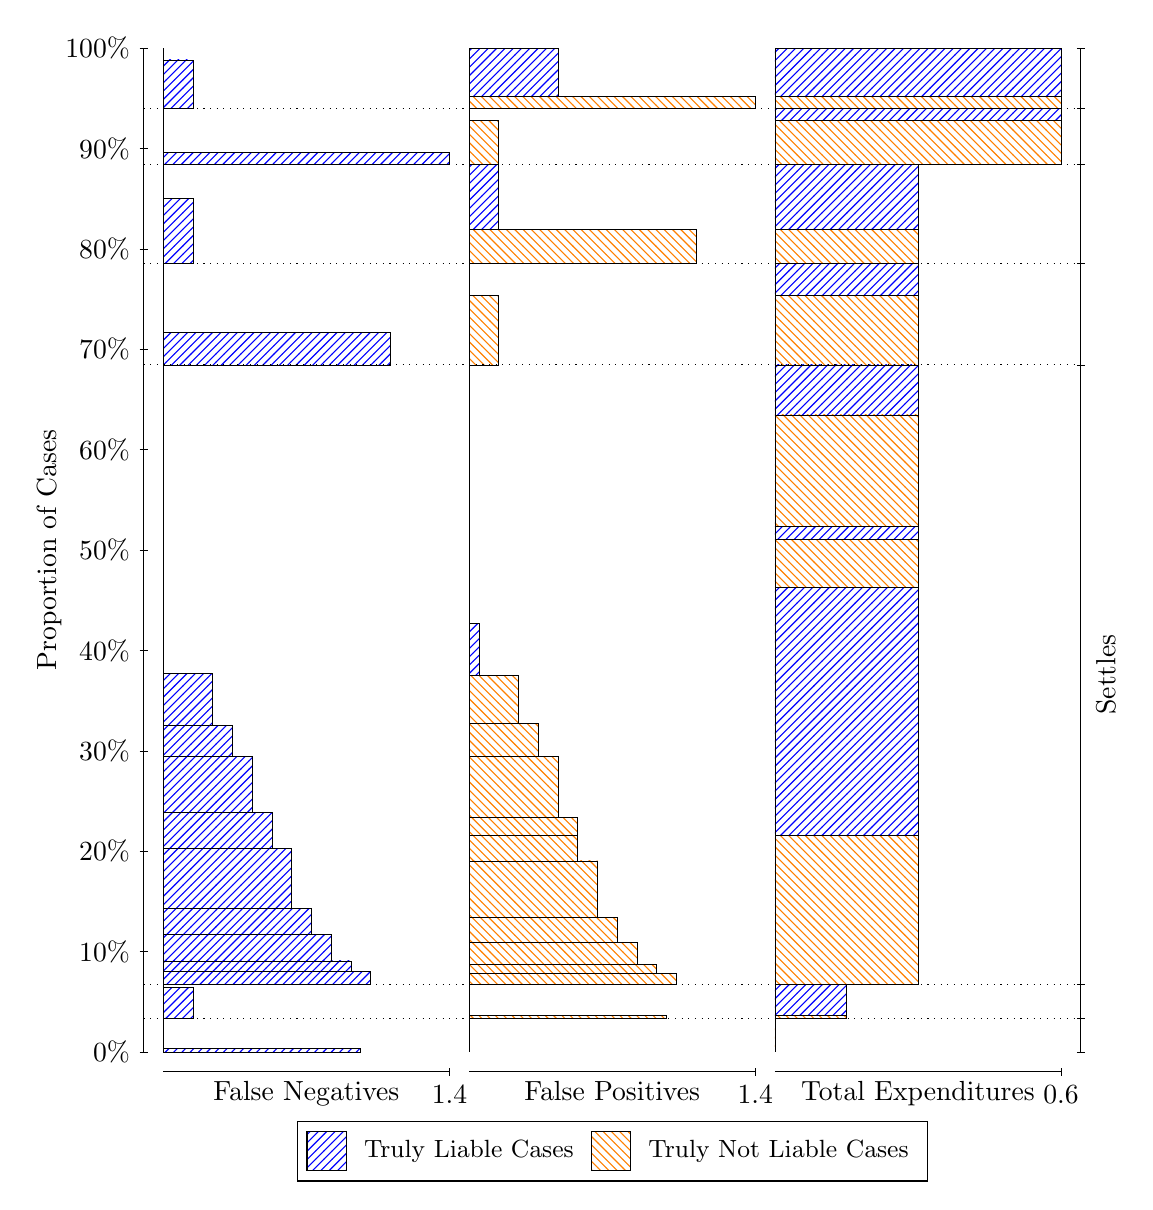
\begin{tikzpicture}
\draw[black, very thin] (1.5,1.75) -- (1.5,14.5);
\node[rotate=90, anchor=center] at (0.3, 8.125) {Proportion of Cases};
\draw[black, very thin] (1.45,1.75) -- (1.55,1.75);
\node[anchor=east] at (1.45, 1.75) {0\%};
\draw[black, very thin] (1.45,3.025) -- (1.55,3.025);
\node[anchor=east] at (1.45, 3.025) {10\%};
\draw[black, very thin] (1.45,4.3) -- (1.55,4.3);
\node[anchor=east] at (1.45, 4.3) {20\%};
\draw[black, very thin] (1.45,5.575) -- (1.55,5.575);
\node[anchor=east] at (1.45, 5.575) {30\%};
\draw[black, very thin] (1.45,6.85) -- (1.55,6.85);
\node[anchor=east] at (1.45, 6.85) {40\%};
\draw[black, very thin] (1.45,8.125) -- (1.55,8.125);
\node[anchor=east] at (1.45, 8.125) {50\%};
\draw[black, very thin] (1.45,9.4) -- (1.55,9.4);
\node[anchor=east] at (1.45, 9.4) {60\%};
\draw[black, very thin] (1.45,10.675) -- (1.55,10.675);
\node[anchor=east] at (1.45, 10.675) {70\%};
\draw[black, very thin] (1.45,11.95) -- (1.55,11.95);
\node[anchor=east] at (1.45, 11.95) {80\%};
\draw[black, very thin] (1.45,13.225) -- (1.55,13.225);
\node[anchor=east] at (1.45, 13.225) {90\%};
\draw[black, very thin] (1.45,14.5) -- (1.55,14.5);
\node[anchor=east] at (1.45, 14.5) {100\%};

\draw[black, very thin] (13.4,1.75) -- (13.4,14.5);
\draw[black, very thin] (13.35,1.75) -- (13.45,1.75);
\node[anchor=west] at (13.35, 1.75) {};
\draw[black, very thin] (13.35,2.172) -- (13.45,2.172);
\node[anchor=west] at (13.35, 2.172) {};
\draw[black, very thin] (13.35,2.6124) -- (13.45,2.6124);
\node[anchor=west] at (13.35, 2.6124) {};
\draw[black, very thin] (13.35,10.476) -- (13.45,10.476);
\node[anchor=west] at (13.35, 10.476) {};
\draw[black, very thin] (13.35,11.768) -- (13.45,11.768);
\node[anchor=west] at (13.35, 11.768) {};
\draw[black, very thin] (13.35,13.021) -- (13.45,13.021);
\node[anchor=west] at (13.35, 13.021) {};
\draw[black, very thin] (13.35,13.736) -- (13.45,13.736);
\node[anchor=west] at (13.35, 13.736) {};
\draw[black, very thin] (13.35,14.5) -- (13.45,14.5);
\node[anchor=west] at (13.35, 14.5) {};

\draw[black, very thin, pattern color=blue, pattern=north east lines] (1.75,1.75) rectangle (4.2557,1.7944);
\draw[black, very thin, pattern color=orange, pattern=north west lines] (1.75,1.7944) rectangle (1.75,2.172);
\draw[black, very thin, pattern color=blue, pattern=north east lines] (1.75,2.172) rectangle (2.1259,2.5663);
\draw[black, very thin, pattern color=orange, pattern=north west lines] (1.75,2.5663) rectangle (1.75,2.6124);
\draw[black, very thin, pattern color=blue, pattern=north east lines] (1.75,2.6124) rectangle (4.381,2.7737);
\draw[black, very thin, pattern color=blue, pattern=north east lines] (1.75,2.7737) rectangle (4.1305,2.906);
\draw[black, very thin, pattern color=blue, pattern=north east lines] (1.75,2.906) rectangle (3.8799,3.2441);
\draw[black, very thin, pattern color=blue, pattern=north east lines] (1.75,3.2441) rectangle (3.6293,3.5758);
\draw[black, very thin, pattern color=blue, pattern=north east lines] (1.75,3.5758) rectangle (3.3787,4.3373);
\draw[black, very thin, pattern color=blue, pattern=north east lines] (1.75,4.3373) rectangle (3.1282,4.7975);
\draw[black, very thin, pattern color=blue, pattern=north east lines] (1.75,4.7975) rectangle (2.8776,5.5029);
\draw[black, very thin, pattern color=blue, pattern=north east lines] (1.75,5.5029) rectangle (2.627,5.8945);
\draw[black, very thin, pattern color=blue, pattern=north east lines] (1.75,5.8945) rectangle (2.3764,6.5551);
\draw[black, very thin, pattern color=orange, pattern=north west lines] (1.75,6.5551) rectangle (1.75,10.476);
\draw[black, very thin, pattern color=blue, pattern=north east lines] (1.75,10.476) rectangle (4.6316,10.886);
\draw[black, very thin, pattern color=orange, pattern=north west lines] (1.75,10.886) rectangle (1.75,11.768);
\draw[black, very thin, pattern color=blue, pattern=north east lines] (1.75,11.768) rectangle (2.1259,12.588);
\draw[black, very thin, pattern color=orange, pattern=north west lines] (1.75,12.588) rectangle (1.75,13.021);
\draw[black, very thin, pattern color=blue, pattern=north east lines] (1.75,13.021) rectangle (5.3833,13.172);
\draw[black, very thin, pattern color=orange, pattern=north west lines] (1.75,13.172) rectangle (1.75,13.736);
\draw[black, very thin, pattern color=blue, pattern=north east lines] (1.75,13.736) rectangle (2.1259,14.349);
\draw[black, very thin, pattern color=orange, pattern=north west lines] (1.75,14.349) rectangle (1.75,14.5);
\draw[black, very thin, pattern color=orange, pattern=north west lines] (5.6333,1.75) rectangle (5.6333,2.1276);
\draw[black, very thin, pattern color=blue, pattern=north east lines] (5.6333,2.1276) rectangle (5.6333,2.172);
\draw[black, very thin, pattern color=orange, pattern=north west lines] (5.6333,2.172) rectangle (8.1391,2.2181);
\draw[black, very thin, pattern color=blue, pattern=north east lines] (5.6333,2.2181) rectangle (5.6333,2.6124);
\draw[black, very thin, pattern color=orange, pattern=north west lines] (5.6333,2.6124) rectangle (8.2644,2.7514);
\draw[black, very thin, pattern color=orange, pattern=north west lines] (5.6333,2.7514) rectangle (8.0138,2.8627);
\draw[black, very thin, pattern color=orange, pattern=north west lines] (5.6333,2.8627) rectangle (7.7632,3.1375);
\draw[black, very thin, pattern color=orange, pattern=north west lines] (5.6333,3.1375) rectangle (7.5126,3.4577);
\draw[black, very thin, pattern color=orange, pattern=north west lines] (5.6333,3.4577) rectangle (7.2621,4.1755);
\draw[black, very thin, pattern color=orange, pattern=north west lines] (5.6333,4.1755) rectangle (7.0115,4.5032);
\draw[black, very thin, pattern color=orange, pattern=north west lines] (5.6333,4.5032) rectangle (7.0115,4.7287);
\draw[black, very thin, pattern color=orange, pattern=north west lines] (5.6333,4.7287) rectangle (6.7609,5.5056);
\draw[black, very thin, pattern color=orange, pattern=north west lines] (5.6333,5.5056) rectangle (6.5103,5.9216);
\draw[black, very thin, pattern color=orange, pattern=north west lines] (5.6333,5.9216) rectangle (6.2598,6.5331);
\draw[black, very thin, pattern color=blue, pattern=north east lines] (5.6333,6.5331) rectangle (5.7586,7.1938);
\draw[black, very thin, pattern color=blue, pattern=north east lines] (5.6333,7.1938) rectangle (5.6333,10.476);
\draw[black, very thin, pattern color=orange, pattern=north west lines] (5.6333,10.476) rectangle (6.0092,11.358);
\draw[black, very thin, pattern color=blue, pattern=north east lines] (5.6333,11.358) rectangle (5.6333,11.768);
\draw[black, very thin, pattern color=orange, pattern=north west lines] (5.6333,11.768) rectangle (8.5149,12.201);
\draw[black, very thin, pattern color=blue, pattern=north east lines] (5.6333,12.201) rectangle (6.0092,13.021);
\draw[black, very thin, pattern color=orange, pattern=north west lines] (5.6333,13.021) rectangle (6.0092,13.585);
\draw[black, very thin, pattern color=blue, pattern=north east lines] (5.6333,13.585) rectangle (5.6333,13.736);
\draw[black, very thin, pattern color=orange, pattern=north west lines] (5.6333,13.736) rectangle (9.2667,13.887);
\draw[black, very thin, pattern color=blue, pattern=north east lines] (5.6333,13.887) rectangle (6.7609,14.5);
\draw[black, very thin, pattern color=orange, pattern=north west lines] (9.5167,1.75) rectangle (9.5167,2.1276);
\draw[black, very thin, pattern color=blue, pattern=north east lines] (9.5167,2.1276) rectangle (9.5167,2.172);
\draw[black, very thin, pattern color=orange, pattern=north west lines] (9.5167,2.172) rectangle (10.425,2.2181);
\draw[black, very thin, pattern color=blue, pattern=north east lines] (9.5167,2.2181) rectangle (10.425,2.6124);
\draw[black, very thin, pattern color=orange, pattern=north west lines] (9.5167,2.6124) rectangle (11.333,4.5032);
\draw[black, very thin, pattern color=blue, pattern=north east lines] (9.5167,4.5032) rectangle (11.333,7.6491);
\draw[black, very thin, pattern color=orange, pattern=north west lines] (9.5167,7.6491) rectangle (11.333,8.2607);
\draw[black, very thin, pattern color=blue, pattern=north east lines] (9.5167,8.2607) rectangle (11.333,8.422);
\draw[black, very thin, pattern color=orange, pattern=north west lines] (9.5167,8.422) rectangle (11.333,9.8404);
\draw[black, very thin, pattern color=blue, pattern=north east lines] (9.5167,9.8404) rectangle (11.333,10.476);
\draw[black, very thin, pattern color=orange, pattern=north west lines] (9.5167,10.476) rectangle (11.333,11.358);
\draw[black, very thin, pattern color=blue, pattern=north east lines] (9.5167,11.358) rectangle (11.333,11.768);
\draw[black, very thin, pattern color=orange, pattern=north west lines] (9.5167,11.768) rectangle (11.333,12.201);
\draw[black, very thin, pattern color=blue, pattern=north east lines] (9.5167,12.201) rectangle (11.333,13.021);
\draw[black, very thin, pattern color=orange, pattern=north west lines] (9.5167,13.021) rectangle (13.15,13.585);
\draw[black, very thin, pattern color=blue, pattern=north east lines] (9.5167,13.585) rectangle (13.15,13.736);
\draw[black, very thin, pattern color=orange, pattern=north west lines] (9.5167,13.736) rectangle (13.15,13.887);
\draw[black, very thin, pattern color=blue, pattern=north east lines] (9.5167,13.887) rectangle (13.15,14.5);
\draw[black, dotted] (1.5,2.172) -- (13.4,2.172);
\draw[black, dotted] (1.5,2.6124) -- (13.4,2.6124);
\draw[black, dotted] (1.5,10.476) -- (13.4,10.476);
\draw[black, dotted] (1.5,11.768) -- (13.4,11.768);
\draw[black, dotted] (1.5,13.021) -- (13.4,13.021);
\draw[black, dotted] (1.5,13.736) -- (13.4,13.736);
\draw[black, very thin] (1.75,1.5) -- (5.3833,1.5);
\node[anchor=north] at (3.5667, 1.5) {False Negatives};
\draw[black, very thin] (5.3833,1.45) -- (5.3833,1.55);
\node[anchor=north] at (5.3833, 1.45) {1.4};

\draw[black, very thin] (5.6333,1.5) -- (9.2667,1.5);
\node[anchor=north] at (7.45, 1.5) {False Positives};
\draw[black, very thin] (9.2667,1.45) -- (9.2667,1.55);
\node[anchor=north] at (9.2667, 1.45) {1.4};

\draw[black, very thin] (9.5167,1.5) -- (13.15,1.5);
\node[anchor=north] at (11.333, 1.5) {Total Expenditures};
\draw[black, very thin] (13.15,1.45) -- (13.15,1.55);
\node[anchor=north] at (13.15, 1.45) {0.6};



\node[black, centered, rotate=90] at (13.72, 6.5441) {Settles};





\draw (7.449999999999999,1.5) node[draw=none] (baseCoordinate) {};
\begin{scope}[align=center]
        \matrix[scale=0.5, draw=black, below=0.5cm of baseCoordinate, nodes={draw}, column sep=0.1cm]{
            \node[rectangle, draw, minimum width=0.5cm, minimum height=0.5cm, pattern=north east lines, pattern color=blue] {}; &
            \node[draw=none, font=\small] (B) {Truly Liable Cases}; &
            \node[rectangle, draw, minimum width=0.5cm, minimum height=0.5cm, pattern=north west lines, pattern color=orange] {}; &
            \node[draw=none, font=\small] (B) {Truly Not Liable Cases}; \\
            };
\end{scope}

\end{tikzpicture}
\end{document}